\chapter{Methodology}
\label{ch:design}

We highlighted two of the factors  that make library building labor intensive and suggest that by automating them we can lift some burden from the library developer. In this chapter, we give more details on how automation can be used for this purpose. 

One of the main components of an algebra library is the axiomatic theory presentation of the algebraic structures, like the different formalizations of \lstmath{Monoid} shown in Figure~\ref{fig:mon-diff-lang}. In some cases, as is mostly the case in theorem provers, developers provide all the declarations of the theory. Another way is to define theories by using combinators which describes how the new theory can be formed in terms of existing ones. 
Combinators are also a useful tool to leverage the structure of the theories by relating them to each other, which is useful when organizing the library as a theory graph. A \emph{flattener} is used to compute the theory and morphisms resulting from the combinator. We discuss our implementation of the flattener in Chapter~\ref{ch:library}. Using these ideas, \lstmath{Monoid} can be defined as 
\begin{togcode} 
Monoid = combine Unital and Semigroup over Magma
\end{togcode} 
Informally, this means that the theory of \lstmath{Monoid} can be constructed by the taking the union of the declarations in \lstmath{Unital}  and \lstmath{Semigroup} without repreating the declarations in \lstmath{Magma}\footnote{The \lstmath{combine} operation is explained in detail in Section~\ref{subsec:combine}}. 

The theories resulting from the flattener are used to compute some universal algebra constructs that are also part of algebra libraries. Chapter~\ref{ch:redundancy} shows examples of homomorphisms, product algebra and term languages provided by library developers. These ones and more can be generated based on their definitions from universal algebra. The \emph{generator} does that by manipulating components of the theories. We discuss the generator in Chapter~\ref{ch:generation}. 

The flattener and generator deal with mathematical definitions while keeping system-specific details to a minimal. In order to make the constructions more useful, the \emph{exporter} makes them available in feature rich systems, like agda. We discuss the exporter in Chapter~\ref{ch:export}. 

Figure~\ref{fig:staged-interpreter} describes the $3$-stage processing that a theory expression goes through. This process make the generation of all the constructions described in Appendix~\ref{appendix:generatedTog} automatically generated from the theory expression of \lstmath{Monoid} above, in both tog and agda. The ideas we present here are not specific to tog and agda and can be applied in a more general scale. 
\begin{figure}
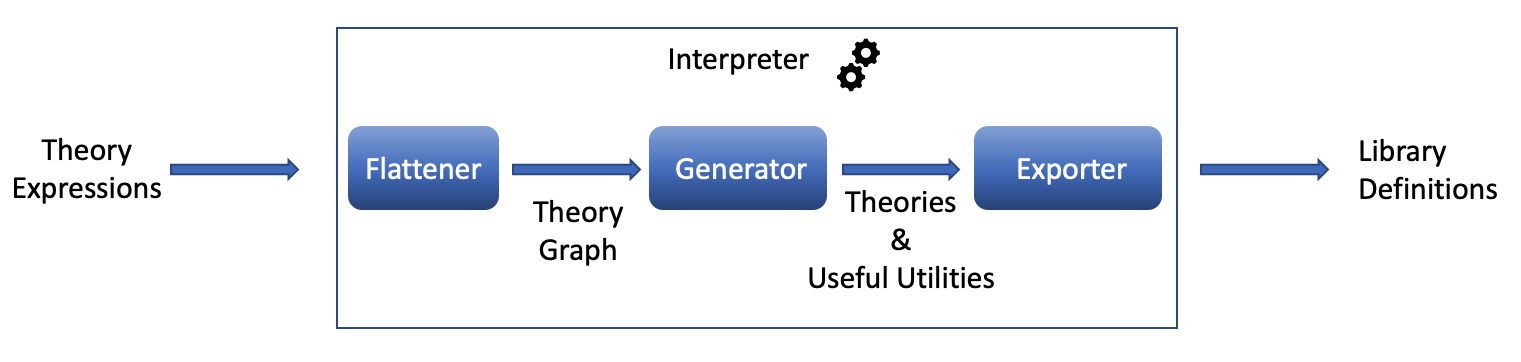
\includegraphics[scale=0.5,width=\linewidth]{figures/interpreter_detailed}
\caption{A $3$-staged interpreter for generating libraries}
\label{fig:staged-interpreter}
\end{figure} 

\begin{comment}
Our work towards adding more automation to theory development envisions users and library developers writing expressions like 
\begin{togcode}
Monoid = combine Unital and Semigroup over Magma
            generate homomorphism, OpenTerms, Simplifier
            using (waist=1,eq=Agda.Builtin.Equality)
\end{togcode}
The systems would then provide the theory presentation for \lstmath{Monoid} as a descendant of \lstmath{Unital} and \lstmath{Semigroup}\ and
the constructions specified in the \lstmath{generate} clause, employing the design decisions in the \lstmath{using} clause.  

The interpreter of the DSL does the transformation from declarative expressions to definitions acceptable by a host language. We suggest an interpreter that consists of three phases as shown in Figure

\paragraph{Flattener.} The first stage of the interpreter builds a theory graph of algebraic structures. To provide more conciseness and better reuse, we use combinators to define new theories. The flattener uses expressions built using the combinators to build a theory graph. The problem here is to choose combinators that leverages the mathematical structure by providing expressive morphisms capable of describing the relationship between theories. We discuss our choice of combinators in Chapter~\ref{ch:library}. A strong requirement that we have regarding combinators is to allow computing flattened theories. While it is useful for the system to know that a \lstmath{Group} is a \lstmath{Monoid} with inverse and automate the transportation of theorems proved in \lstmath{Monoid} theory to be used in \lstmath{Group} theory, some potential users might want to use \lstmath{Group}s without caring about how they are built. We want to use combinators that allows both views for users, by avoiding qualified names and dropping and freeness combinators.\ednote{probably need references here.}
%without imposing one of Our library need to support both definitions, by enabling the users to work with flat version of the library. Some operations on theories make this hard to achieve, like dropping and freeness combinators by CASL\ednote{look for a source explaining why they are problematic}. 

\paragraph{Generator.} The input to the generator is a flat theory presentation, the output of the flattener. The generator manipulates the components of a theory presentation generating related constructions based on how they are defined in universal algebra. Therefore, the input theory needs to fit in the universal algebra abstraction of a theory, being a first-order equational theory. Despite this limitation, the algebraic hierarchy until at least \lstmath{Ring}\ednote{or maybe more?} fits in this criteria. 
We discuss our implementation of the generator in Chapter~\ref{ch:generation}. 

\paragraph{Exporter.} 
\end{comment} 

